\documentclass[11pt]{article}
\usepackage[utf8]{inputenc}
\usepackage[ngerman]{babel}
\usepackage[T1]{fontenc}
\usepackage{csquotes}
\usepackage{hyperref}
\usepackage{booktabs}
\usepackage{a4wide}
\usepackage{graphicx}
\usepackage{biblatex}
\usepackage{amsmath}
\usepackage{amssymb}
\usepackage{listings, listings-rust}
\usepackage{xcolor}

\definecolor{codegreen}{rgb}{0,0.6,0}
\definecolor{codegray}{rgb}{0.5,0.5,0.5}
\definecolor{codepurple}{rgb}{0.58,0,0.82}
\definecolor{backcolour}{rgb}{0.95,0.95,0.92}

\lstdefinestyle{mystyle}{
    backgroundcolor=\color{backcolour},   
    commentstyle=\color{codegreen},
    keywordstyle=\color{magenta},
    numberstyle=\tiny\color{codegray},
    stringstyle=\color{codepurple},
    basicstyle=\ttfamily\footnotesize,
    breakatwhitespace=false,         
    breaklines=true,                 
    captionpos=b,                    
    keepspaces=true,                 
    numbers=left,                    
    numbersep=5pt,                  
    showspaces=false,                
    showstringspaces=false,
    showtabs=false,                  
    tabsize=2
}

\lstset{style=mystyle}

\addbibresource{bibliography.bib}
\pagestyle{plain}

\title{Live Programmierung technoider Meditationsmusik mit analogem Synthesizer}
\author{Patrick Simmelbauer \and Lukas Zahel \and Phil Krause}

\date{20. Juli 2026}

\begin{document}

\maketitle

\section{Einleitung}
Tidal \cite{mclean2010tidal}

\subsection{Idee und Konzept}

Die Motivation für das vorliegende Projekt entstand im Rahmen einer Yoga-Klangbad-Sitzung. Dabei werden sphärische Klangflächen eingesetzt, um Teilnehmende in einen mental entspannten, meditativen Zustand zu versetzen. Zentrales klangliches Mittel dieser Praxis sind Schwebungen. Sie entstehen durch die Überlagerung zweier minimal frequenzverschobener Töne und erzeugen periodische Lautstärkeschwankungen.

Ein strukturell verwandtes Phänomen lässt sich im Techno beobachten. Durch repetitive rhythmische Muster, wird ebenfalls ein tranceartiger, meditativer Wahrnehmungszustand erzeugt. Der Mechanismus ist hier jedoch primär rhythmisch statt harmonisch-klanglich. Das harmonische Schwebungsprinzip des Klangbads und das rhythmische Wiederholungsprinzip des Techno zielen somit auf einen ähnlichen psychoakustischen Effekt. Sie unterscheiden sich jedoch in ihrer klanglichen Umsetzung.

Ziel des vorliegenden Projekts ist es, Elemente beider Konzepte in einer gemeinsamen Komposition zu verbinden. Als musikalische Orientierung dient dabei das Genre Ambient Techno. Es verbindet bereits ambiente, flächige Klangtexturen mit repetitiven, technoiden Rhythmusstrukturen.

Zur technischen Umsetzung wird das Live-Coding-Framework Tidal Cycles eingesetzt. Es wird um mehrere externe Hardware- und Softwarekomponenten erweitert: ein MIDI-Interface, einen analogen Synthesizer, ein MIDI-Keyboard sowie eine modulare Synthesizer-Software. Der Einsatz dieser externen Systeme verfolgt vier Ziele. Erstens soll die technische Machbarkeit und Praxistauglichkeit ihrer Anbindung an Tidal Cycles untersucht werden. Zweitens soll die gleichzeitige Partizipation mehrerer Anwender:innen am Kompositionsprozess ermöglicht werden. Drittens soll durch die Kombination unterschiedlicher Klangquellen ein höheres Maß an spontaner klanglicher Varianz erzeugt werden, als dies mit einer rein softwarebasierten Lösung möglich wäre. Viertens wird ein analoger Synthesizer eingebunden, da analoge Klangerzeugung ein stilprägendes Element des Ambient Techno darstellt.

Formal folgt der Songaufbau einem Spannungsbogen von Ruhe zu Komplexität und zurück. Der Song beginnt mit einer elektronisch nachgebildeten Klangbad-Textur. Diese verdeutlicht einleitend die entspannende Wirkung der Schwebungen. Im Verlauf des Stücks findet ein gradueller Übergang von diesen ruhigen Schwebungen hin zu technoiden Rhythmusmustern statt. Dabei werden typische stilistische Elemente des Ambient Techno integriert. Die Komplexität der Komposition nimmt kontinuierlich zu. Gegen Ende des Stücks kehrt sie wieder zu den einleitenden Schwebungen zurück. Diese bilden während der gesamten Spieldauer das klangliche Fundament.

Das entstandene Musikstück dient somit als klangliches Fallbeispiel für zwei unterschiedliche musikalische Methoden, Schwebung und rhythmische Repetition. Mittels dieser Methoden können tranceartige Wahrnehmungszustände sowie eine sphärische Klangästhetik erzeugt werden.

\subsection{Techno}

1989 markiert das Jahr, in dem das Musikgenre Techno erstmals eine breite öffentliche und kulturelle Wahrnehmung erlangte \cite{ischebeck_subjekt_2025}. Techno ist ein überwiegend instrumentales Musikgenre, das sich im Laufe seiner Entwicklung stark ausdifferenziert hat \cite{hecken_techno_2017}. Charakteristisch zeichnet es sich durch drei zentrale Merkmale aus: ein hohes Tempo ab circa 120 Beats pro Minute mit einer kontinuierlichen Bassdrum in Viervierteltakt („Four to the Floor”), die additive Überlagerung repetitiver perkussiver und melodischer Patterns und der Einsatz elektronisch erzeugter und häufig bewusst hart und technisch klingender Sounds \cite{hecken_techno_2017}. Die Produktion verfolgt einem szenebasierten Do-It-Yourself-Ansatz (DIY) und wird mit Computer, elektronischen Instrumenten wie Drum Machines und Synthesizer sowie Samplern produziert \cite{hecken_techno_2017}.

\subsection{Ambient}

Ambient-Musik stellt ein Subgenre der elektronischen Musik dar, dessen Ursprünge sich in der ersten Hälfte des 20. Jahrhunderts verorten lassen. \cite{velescu_ambient_2015} 
Als Form atmosphärischer Hintergrundmusik konzentriert sich das Genre weniger auf melodische und rhythmische Entwicklung, als auf Klangfarben und die Schaffung eines bestimmten Klangraums.  \cite{velescu_ambient_2015}

Charakteristische Merkmale des Genres sind die bevorzugte Verwendung von Dur- oder pentatonischer Tonleitern, eine stark reduzierte, minimalistische Klangplatte und eine geringe harmonische Komplexität. Auf Gesang und perkussive Elemente wird weitestgehend verzichtet. Häufig werden organisch wirkende Klangfarben mit Naturaufnahmen kombiniert, welche durch einen ausgeprägten Hall-Effekt eine räumliche und atmosphärische Wirkung erhalten. \cite{burdon_immunological_2023}

\subsection{Ambient Techno}
TODO: Überarbeiten und Quellen recherchieren!

Ambient Techno bildet die Schnittmenge der beiden zuvor beschriebenen Genres: Es verbindet die atmosphärischen, klangfarbenorientierten Klangtexturen des Ambient mit den rhythmischen und produktionstechnischen Mitteln des Techno (Wikipedia: Ambient techno, o. J.). Zu den prägenden Künstler:innen zählen B12, Aphex Twin und Biosphere (AllMusic: Ambient Techno, o. J.). Stilistisch verbindet das Genre die melodischen und rhythmischen Ansätze von Techno und Electro mit den schwebenden, vielschichtigen, aquatischen Atmosphären des beatlosen und experimentellen Ambient: Eingesetzt werden techno-typische 808- und 909-Drumcomputer, dünn klingende Elektronik sowie Melodien in Moll und fremdartig klingende Samples (AllMusic: Ambient Techno, o. J.).

\section{Hard- und Software-Aufbau}

\begin{figure}[htbp]
    \centering
    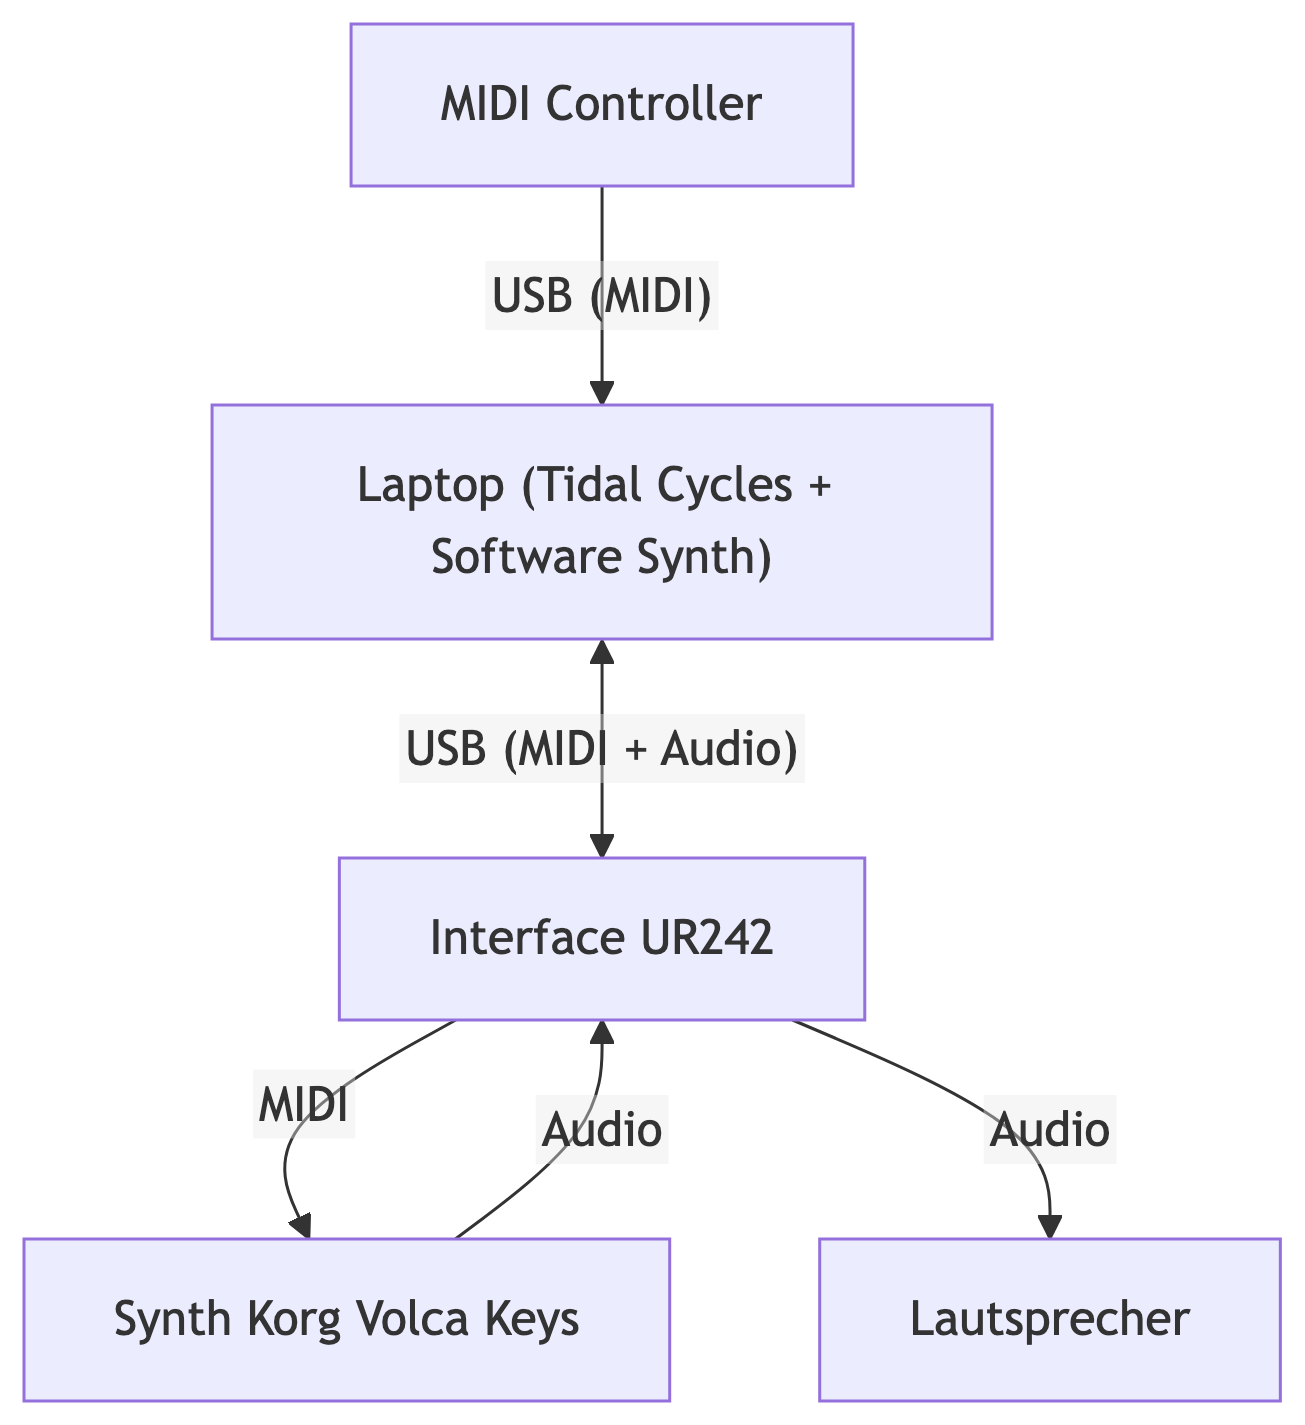
\includegraphics[height=250pt]{../assets/setup.png}
    \caption{Hard- und Software-Aufbau des Projekts}
    \label{fig:setup}
\end{figure}

Im Projekt werden drei verschiedene Tonquellen genutzt. Dabei tauschen die Tonquellen untereinander Steuersignale aus und müssen am Ende zu einem einzelnen Tonsignal zusammengeführt werden. Da eine der Tonquellen ein externer Hardware-Synthesizer ist, reicht eine softwareseitige Verbindung nicht aus, und es ist zusätzliche Hardware notwendig. Eine Übersicht über die Verkabelung der Hardware-Komponenten ist in Abbildung \ref{fig:setup} dargestellt.

Das Herzstück des Aufbaus stellt das Audio- und MIDI-Interface \textit{Steinberg UR242} dar. Dieses wird per USB-Anschluss mit dem Laptop verbunden und ermöglicht das Anbinden von externen Audio- und MIDI-Geräten. Das Interface kann dann im Betriebssystem als Audioausgabegerät genutzt werden. Das empfangene digitale Audiosignal wird im Interface in ein analoges Signal umgewandelt. Das analoge Ausgangssignal des Interfaces wird direkt mit dem Lautsprecher-Aufbau verbunden.

Zur Modulierung verschiedener Parameter des Software-Synthesizers wird ein \textit{AKAI MPK mini}~\cite{AkaiMPKMiniMK3} verwendet. Dieses MIDI-Keyboard, das mit einer Klaviatur und verschiedenen Drehreglern ausgestattet ist, ist in der Lage, MIDI-Signale über eine USB-Schnittstelle zu versenden. In diesem Projekt kommen jedoch lediglich die Drehregler zum Einsatz. Diese versenden ein MIDI-Control-Change-Signal (MIDI-CC) (vgl. Abschnitt \ref{sec:MIDI}).

\subsection{Tonquellen}

Im folgenden Abschnitt werden die drei im Projekt verwendeten Tonquellen näher beschrieben. Dabei wird auf die Funktionsweise der Tonquellen eingegangen sowie erläutert, wie diese Instrumente im Projekt eingesetzt werden.

\subsubsection{Korg Volca Keys}
Der im Projekt verwendete externe Synthesizer ist der \textit{Korg Volca Keys}. Sein MIDI-Eingang wird mit dem MIDI-Ausgang des Audio-Interfaces verbunden. Welche Noten zu welchem Zeitpunkt vom Synthesizer wiedergegeben werden sollen -- oder anders ausgedrückt, welche Frequenzen die analogen Oszillatoren in ihm erzeugen sollen -- wird über die MIDI-Schnittstelle gesteuert. Das dabei erzeugte Audiosignal wird zurück zum Interface geleitet und dort in ein digitales Signal umgewandelt, das der Laptop verarbeiten kann.

Der Korg Volca Keys ist ein analoger Synthesizer, der über drei Oszillatoren verfügt. Im Projekt wird er im Modus \textit{UNISON} betrieben. In diesem Modus erzeugen die drei Oszillatoren des Synthesizers eine Sägezahnschwingung mit identischer Frequenz. Dies erzeugt einen volleren Klang als ein einzelner Oszillator. Zusätzlich kann durch den \textit{DETUNE}-Regler die Frequenz eines der Oszillatoren leicht verändert werden. Auch dadurch entstehen Schwebungen (vgl. Abschnitt \ref{sec:schwebung}), die im Projekt als zentrales klangliches Mittel eingesetzt werden.

Der Synthesizer verfügt über einen Tiefpassfilter, der auch über den internen LFO moduliert werden kann. Ebenso sind die \textit{ATTACK}-, \textit{DECAY/RELEASE}- sowie \textit{SUSTAIN}-Parameter des internen Hüllkurvengenerators über drei der verbauten Potentiometer einstellbar. Im Projekt wird zusätzlich der interne Delay-Effekt des Synthesizers genutzt. Dieser kann über die \textit{TIME}- und \textit{FEEDBACK}-Regler eingestellt werden.

\subsubsection{Software-Synthesizer}

Neben dem Hardware-Synthesizer wird im Projekt ein Software-Synthesizer genutzt. Dieser ist über eine Browser-Oberfläche konfigurierbar und kann über die Web-MIDI-API~\cite{Wilson:25:WMA} angesprochen werden. Das erzeugte Tonsignal wird über das Betriebssystem an das Audio-Interface geleitet.

\begin{figure}[htbp]
    \centering
    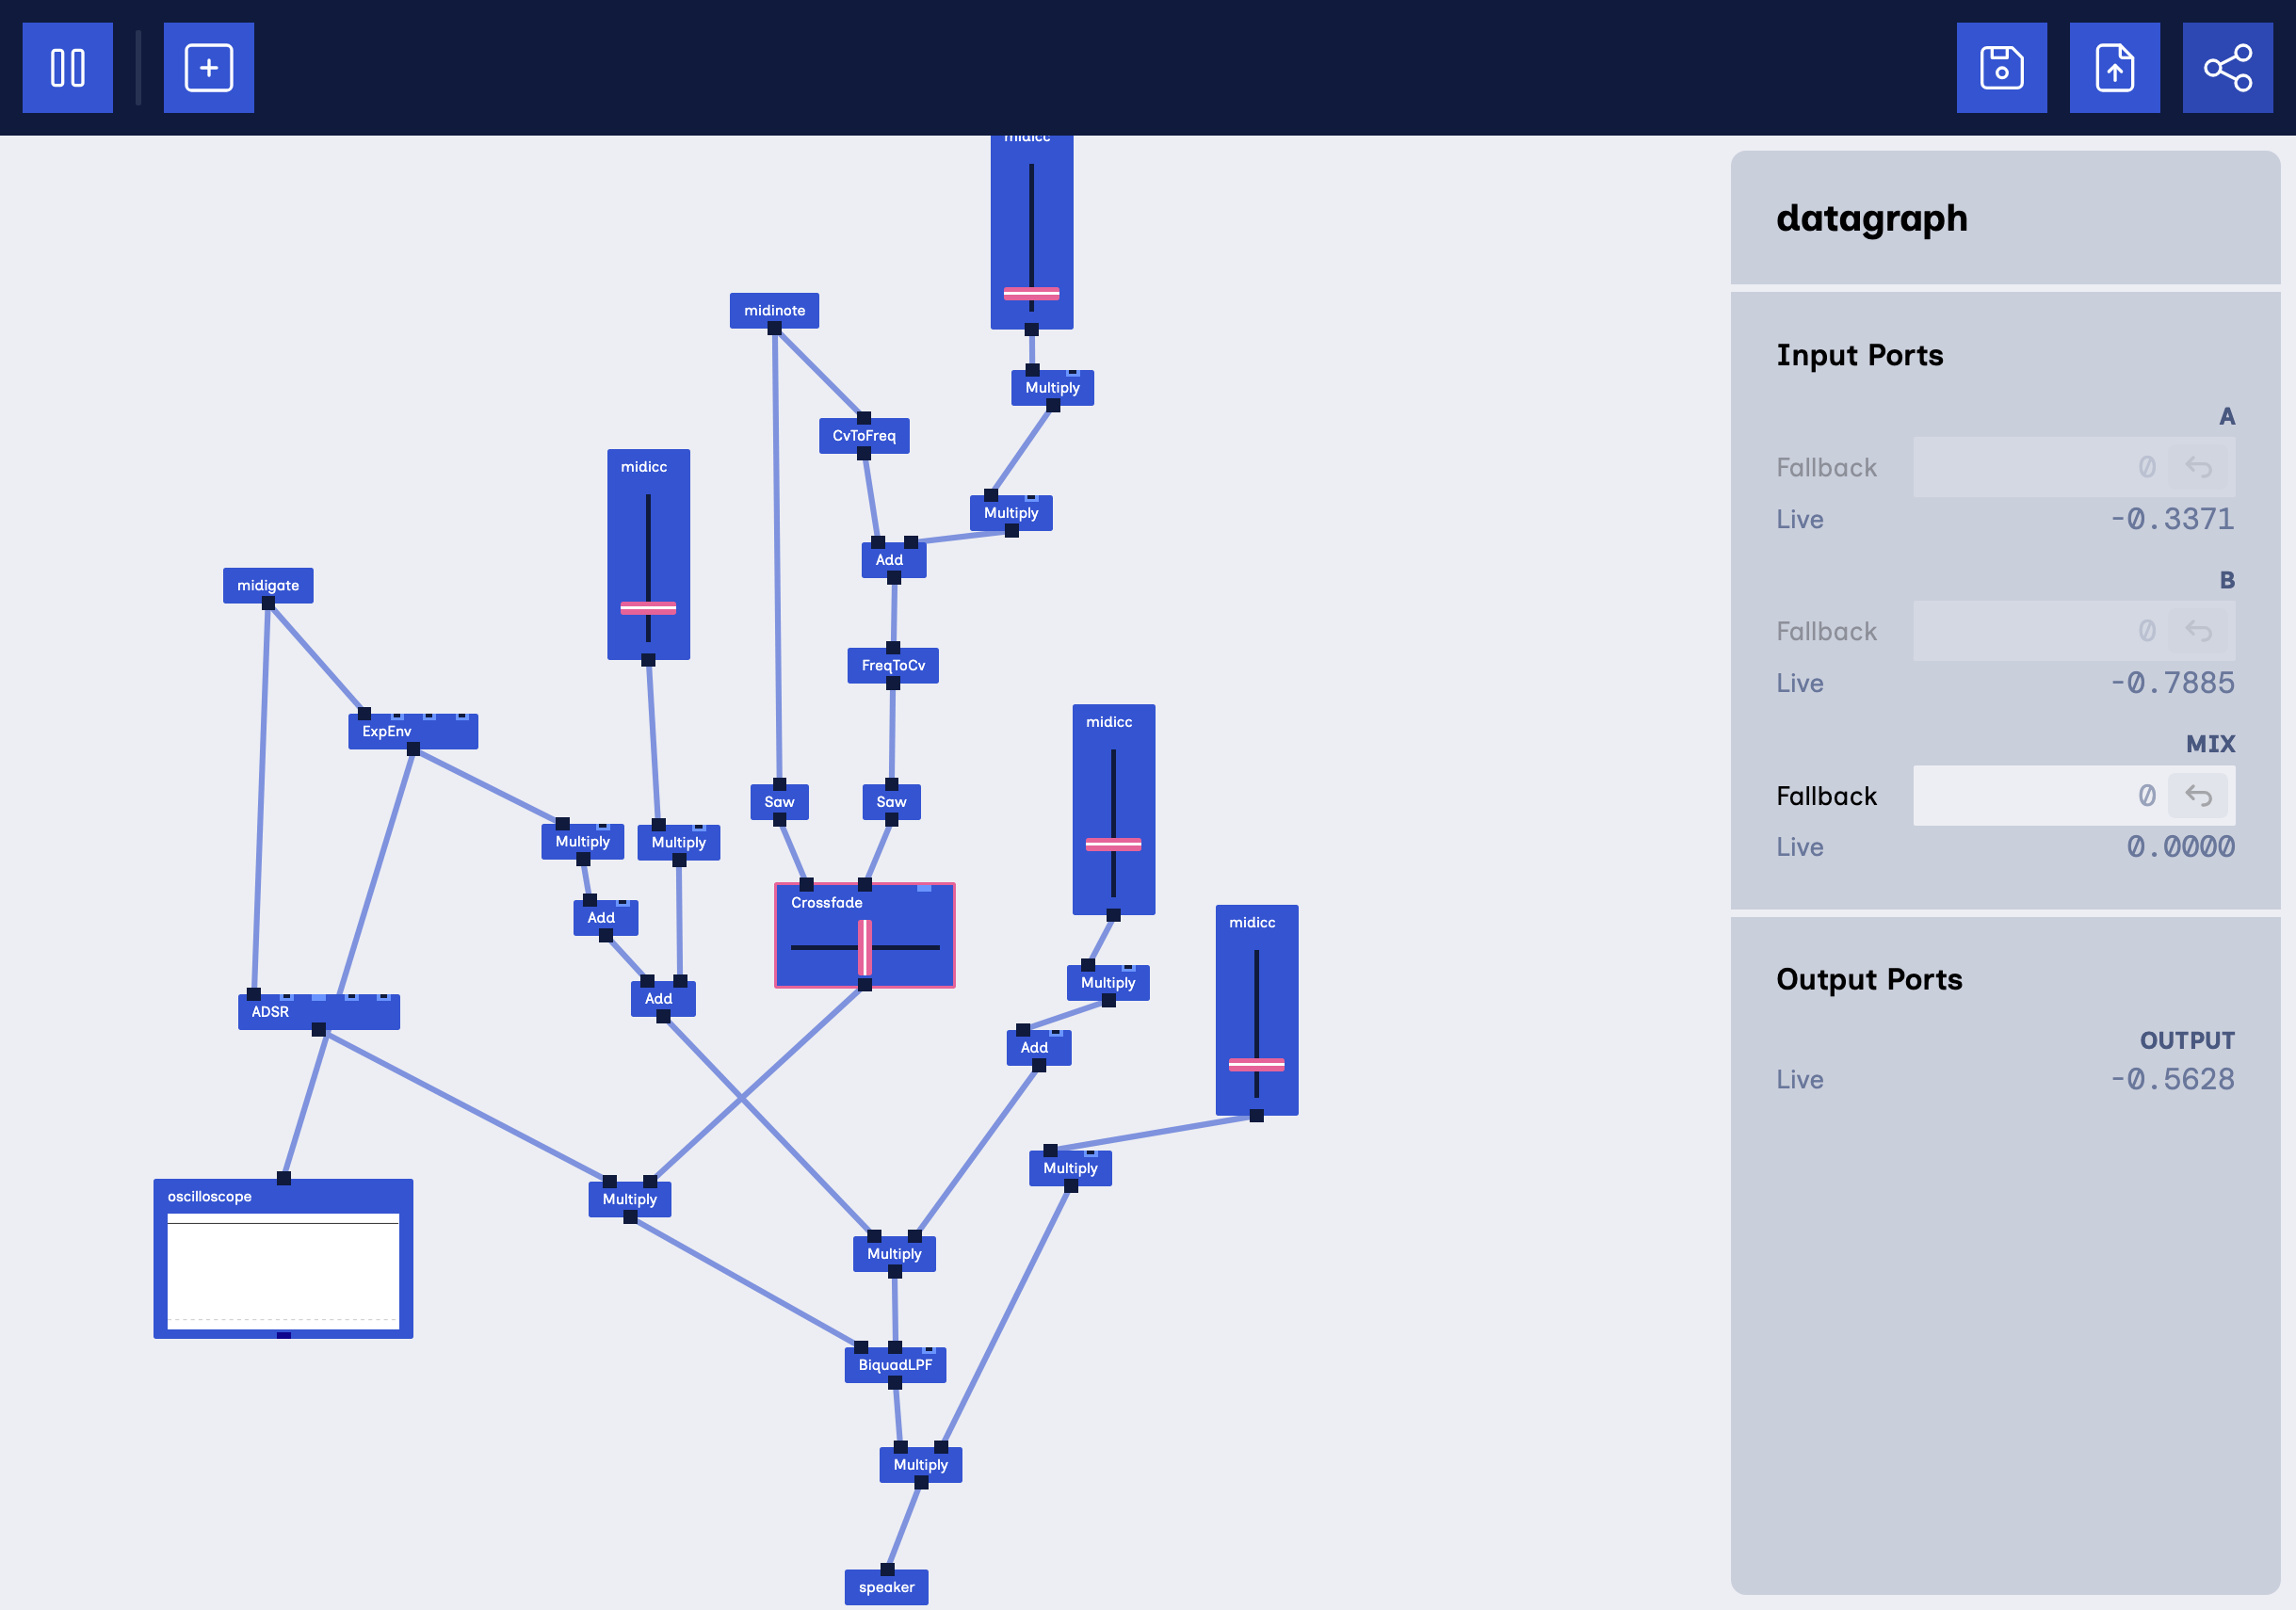
\includegraphics[height=250pt]{../assets/datagraph.png}
    \caption{Ein Patch in der Software-Synthesizer-Umgebung}
    \label{fig:datagraph}
\end{figure}

Der Software-Synthesizer erzeugt Töne durch einen vom Nutzer programmierbaren Audio-Graph. Der Audio-Graph besteht aus Knoten, die miteinander verbunden werden können. Jeder Knoten hat eine bestimmte Funktion, wie z.B. die Erzeugung eines Tonsignals, die Modulation eines Signals oder die Addition von Signalen. Codebeispiel \ref{lst:add} zeigt eine einfache Implementierung eines Knotens, der zwei Eingangssignale addiert und das Ergebnis an einem Ausgang bereitstellt. Im Codebeispiel \ref{lst:add_example} ist zu sehen wie dieser Add-Knoten dann programmatisch via Rust API genutzt werden kann. Hier werden 2 Sinus Signale unterschiedlicher Frequenzen addiert und die ersten 10 generierten Sample-Werte ausgegeben.

Im Projekt benutzen wir jedoch nicht die Rust API direkt, sondern nutzen eine graphische Nutzeroberfläche mit welcher man Audio-Graphen dieser Art visuell erstellen kann. Abbildung \ref{fig:datagraph} zeigt die visuelle Darstellung eines Audio-Graphin in der Nutzeroberfläche.


\begin{lstlisting}[language=rust, caption=Implementierung eines Knotens zur Addition in der Software-Synthesizer-Umgebung, label=lst:add]
pub struct Add;
impl Node<2, 1> for Add {
  const INPUT_NAMES: [&'static str; 2] = ["input1", "input2"];
  const OUTPUT_NAMES: [&'static str; 1] = ["output"];
  const CATEGORY: &'static str = "math";
  fn process(&mut self, input: [f32; 2], output: &mut [f32; 1]) {
    output[0] = input[0] + input[1];
  }
  fn new(_: u32) -> Self {
    Self
  }
}
\end{lstlisting}

\begin{lstlisting}[language=rust, caption=Beispielhafte Nutzung des Add-Knotens in der Software-Synthesizer-Umgebung, label=lst:add_example]
let mut graph = Graph::new(44100);
let freq1 = graph.add_param(Frequency::from_hz(440.0).cv());
let freq2 = graph.add_param(Frequency::from_hz(880.0).cv());
let sin1 = graph.add::<Sin>();
let sin2 = graph.add::<Sin>();
let add = graph.add::<Add>();

// 440 Hz -> sin1
let _ = graph.connect_ports(&freq1.output_port(0).unwrap(), &sin1.input_port(0).unwrap());
// 880 Hz -> sin2
let _ = graph.connect_ports(&freq2.output_port(0).unwrap(), &sin2.input_port(0).unwrap());

// sin1 + sin2 -> add
let _ = graph.connect_ports(&sin1.output_port(0).unwrap(), &add.input_port(0).unwrap());
let _ = graph.connect_ports(&sin2.output_port(0).unwrap(), &add.input_port(1).unwrap());

for _ in 0..10 {
  let value = *graph.port_value(&add.output_port(0).unwrap()).unwrap();
  println!("{:?}", value);
  graph.tick();
}

/*
Output:
  0.0
  0.07453336
  0.26173612
  0.4460045
  0.625177
  0.7971648
  0.95998126
  1.1117709
  1.2508352
  1.3756568    
*/
\end{lstlisting}


\subsubsection{SuperCollider}
Als dritte und letzte Tonquelle wird im Projekt \textit{SuperCollider}~\cite{mccartney1996supercollider} genutzt. SuperCollider dient als Backend für TidalCycles: TidalCycles steuert SuperCollider, SuperCollider erzeugt Audio- und MIDI-Signale und leitet diese an die jeweiligen Hard- und Software-Geräte weiter. Konkret erzeugt SuperCollider im Projekt die perkussiven Elemente und nutzt dafür Samples und Synthesizer, die mit der Installation von \textit{TidalCycles} mitgeliefert werden.

%----------------------------
% Phils Sachen
%--------------------------
\section{Theorie}
\subsection{Schwebung}
Zwei Schwingungen mit gleicher Amplitude und leicht unterschiedlichen Frequenzen, werden vom menschlichen Ohr nicht als zwei getrennte Töne wahrgenommen, stattdessen hört man einen Ton einer Frequenz die genau zwischen den beiden ursprünglichen Tönen liegt, dieser wird jedoch kontinuierlich lauter und wieder leiser. Dieser Effekt ist allgemein als Schwebung bekannt. Der Effekt ergibt sich direkt aus der Addition der beiden Schwingungen.
\begin{equation}
    \label{eq:Addition}
    A_{res}(t) = A \sin(2\pi f_1t) + A \sin(2\pi f_2t)
\end{equation}
Es gilt:
\begin{equation}
    \label{eq:Trig}
   \sin(a) + \sin(b) = 2\sin(\frac{a+b}{2})\cos(\frac{a-b}{2})
\end{equation}
Durch Einsetzen von \ref{eq:Trig} in \ref{eq:Addition} folgt dann:
\begin{equation}
    \label{eq:Ergebnis}
    \begin{aligned}
        A_{res}(t) = 2 A \cos(2\pi \frac{f_1-f_2}{2}t) \sin(2\pi \frac{f_1+f_2}{2}t) \\
            = 2 A \cos(\pi f_{Schwebung}t) \sin(2\pi f_r t)
    \end{aligned}
\end{equation}
Wobei $\frac{f_1+f_2}{2}$ die Frequenz des resultierenden Tones $f_r$ beschreibt und $\frac{f_1-f_2}{2}$ die Frequenz mit der sich die Amplitude ändert. Da nur der Betrag der Amplitude interessant ist, schreiben wir $f_{Schwebung} = |f_1 - f_2|$.
Der Effekt der Schwebung kann zur Klangsynthese ausgenutzt werden, insbesondere bei der Verwendung gleicher Töne, von denen einer eine leichte Frequenzveränderung erfährt ist die resultierende Schwebungsfrequenz direkt abhängig von der Änderung der Frequenz:
\begin{equation}
    \begin{gathered}
    f_{Schwebung} = |f_1 - f_2| \\
    f_2 = f_1 + f_{shift} \\
    f_{Schwebung} = |f_1 - (f_1 + f_{shift})| = |f_{shift}|
    \end{gathered}
\end{equation}
Durch diese Eigenschaft können sehr gezielt Schwebungsfrequenzen erzeugt werden, die beispielsweise zum Takt der Musik passen.


\subsection{Sägezahn-Schwingung}
Gleichung \ref{eq:Saegezahn} zeigt die Fourier-Zerlegung einer Sägezahnschwingung bekannt aus der Vorlesung und Übung.
\begin{equation}
    \label{eq:Saegezahn}
    f = - \frac{2}{\pi}\sum_{k\geq1}\frac{(-1)^k}{k}\sin(kx)
\end{equation}
Aus der Gleichung folgt, das eine Sägezahnschwingung aus einer Grundfrequenz und deren ganzahligen Vielfachen zusammengesetzt wird. Wird auf eine solche Schwingung nun ein sogenannter Tiefpassfilter angewendet, dessen Filterfrequenz sich der Grundfrequenz der Sägezahnschwingung annähert $(f_{filter} \to x)$, so ensteht wiederum eine reine harmonische Schwingung, da nur die Grundfrequenz übrig bleibt und die vielfachen gefiltert werden. Aufgrund des unterschiedlichen Klangbilds einer Sägezahnschwingung im Vergleich zu einer rein harmonischen Schwingung kann dieser Effekt ausgenutzt werden, um den Klang eines Synthesizers anzupassen.\\
Die durch einen Synthesizer erzeugte Sägezahnschwingung wird hierbei durch einen Tiefpassfilter geleitet, um so höher die eingestellte Filterfrequenz ist, desto mehr gleicht die resultierende Schwingung dem Original, der Ton klingt also, typisch für Sägezahnschwingungen, rau, $f_{filter} \to \infty$ wäre hierbei die perfekte Sägezahnschwingung. Je mehr die Filterfrequenz nun der Grundfrequenz des erzeugten Tons angenähert wird, desto weicher klingt der resultierende Ton.

\subsection{Delay}

\section{Ablauf des Live-Konzerts}
Das gesamte Konzert findet in einer Geschwindigkeit von 128 Schlägen pro Minute statt. Dies wird erreicht indem zu Beginn einmal der Befehl $setcps (128/60/4)$ ausgeführt wird. Das Konzert beginnt mit dem Klang von zwei Klangschalen des gleichen Tones. Anschließend wird der Klang einer der beiden Klangschalen mit dem $fshift$ Effekt von TidalCycles modifiziert. Durch die leichte Frequenzverschiebung einer der beiden Töne entsteht eine Schwebung (siehe Abschnitt~\ref{sec:schwebung}). Der Effekt ist dabei so eingestellt, das eine Frequenzverschiebung von $k \cdot \frac{128}{60}$ mit $k \in \mathbb{N}$ stattfindet. Dadurch wird eine Schwebungsfrequenz erzeugt, die ein ganzzahliges Vielfaches der Taktrate beträgt. Die Wellenbäuche bzw. -Knoten der Schwebung passen damit zum Takt der Musik. Die Umsetzung in TidalCycles ist in Listing~\ref{lst:tidal-schwebung} zu sehen. Die Funktion $gong$ erzeugt hierbei zwei Töne von welchen einer mit dem $fshift$ Effekt modifiziert wird. Der Parameter $shift$ entspricht dabei dem oben genannten $k$ und kann beliebig verändert werden, um die gewünschte Schwebungsfrequenz zu erzeugen.

\begin{lstlisting}[language=Haskell, caption={Erzeugung von $supergong$-Tönen mit Parametrisierung der Schwebungsfrequenz.}, label={lst:tidal-schwebung}]
let bpm = 128
setcps (bpm/60/4)

gong shift = stack [ slow 2 $ n (scale "hexSus" "f3") # s "supergong"
                   , slow 2 $ n (scale "hexSus" "f3") # s "supergong" # fshift (shift * bpm/60)
                   ]

d1 $ gong 2 # gain 0.6
\end{lstlisting}

Nun werden geschlossene Highhats hinzugefügt, welche mit einem Tiefpassfilter moduliert werden. Die Filterfrequenz wird hierbei mit einem Sinus der halben Schwebungsfrequenz geändert.

Nun wird ein eigens konstruierter Bass zugeschalten, dieser wurde mithilfe des Software-Synthesizers, der in Abschnitt~\ref{sec:softwaresynth} beschrieben wird, modular zusammengebaut und besteht aus zwei Sägezahnschwingungen und besitzt verschiedene Parameter welche über Drehknöpfe des MIDI-Keyboards, angepasst werden können (vgl. Abschnitt~\ref{sec:MIDI}).

%TODO: Erklärung aller Parameter ergänzen / genauer formulieren (vor allem Acidität)
Die vier einstellbaren Parameter sind eine Frequenz-Verschiebung einer der beiden Sägezahnschwingungen (ähnlich wie bei Klangschale um $k \cdot \frac{128}{60}$) um eine gezielte Schwebung zu erzeugen, ein Tiefpassfilter mithilfe welchem der Klang zwischen Sägezahn und harmonischer Schwingung verändert werden kann (vgl. Abschnitt \ref{sec:sawtooth}), ein Lautstärke-Regler und eine Einstellung mit welcher ein Filter der wiederum an den Attack-Wert der beiden Schwingungen gebunden ist eingestellt werden kann.

Der Bass wird zunächst mit einem Filterwert nahe der Grundfrequenz des Tons und einer Schwebung gleich der der Klangschalen verwendet. Nun wird zunächst ein Filter auf die Klangschalen angewendet bevor diese ganz entfernt werden.

Verschiedene Schlag-Elemente werden zugeschaltet, sowie der \textit{Korg Volca Keys}-Synthesizer, dieser spielt zunächst jedoch nur einzelne Töne zu Beginn jedes zweiten Taktes und keine Melodie. Durch Einstellen eines hohen Delay-Feedbacks und Veränderung der Zeit-Komponente wird eine Art Tremolo mit schwankender Tonhöhe erzeugt (siehe Abschnitt \ref{sec:delay}). \\

%TODO: warum hexSus und warum diese Töne, bringt der lpf wirklich was?? %
Ein Pad wird aus drei zyklisch wechselnden Akkorden innerhalb der hexSus-Skala erstellt (Vergleich Listing~\ref{lst:tidal-pad}). Das Pad erzeugt Hintergrundtextur und fügt gleichzeitig eine melodische Ebene hinzu.
Eine lange Attack-Zeit von drei Sekunden sowie eine Release-Zeit von fünf Sekunden sorgt dafür, dass die Akkorde ohne hörbaren Einsatzpunkt einschwingen und weich ineinander übergehen. In Kombination mit \texttt{legato 2} überlappen sich aufeinanderfolgende Akkorde zeitlich, sodass der perkussive Charakter eines klassischen Akkordanschlags vermieden wird. Ein stark ausgeprägter Reverb (\texttt{room 0.9}, \texttt{size 0.95}) verleiht dem Pad abschließend die räumliche Tiefe für den sphärischen Gesamtklang.

\begin{lstlisting}[language=Haskell, caption={Erzeugung Hintergrund Pad}, label={lst:tidal-pad}]
d3 $ slow 2 $ n ( scale "hexSus" "<[-2, 1, 5] [1, 3, 4, 7] c'min>") # s "superzow"
  # attack 3                            
  # release 5
  # sustain 1
  # legato 2
  # lpf (slow 20 $ range 400 "2000" $ sine)
  # room 0.9 # size 0.95
  # gain 0.6
\end{lstlisting}

\begin{enumerate}
    \item Einstellung Synthi "Acid" (rauer Ton durch hohe LFO Frequenz)
    \item Random Töne Synthi
    \item Abbau und Rückkehr zu Schwebung
\end{enumerate}

\printbibliography

\end{document}
